% % \part{数学建模实战}
% % \chapter{血管重建}

% \documentclass[UTF8]{ctexbook}

% \ctexset{
%     part/number = \chinese{part}
% }

% \usepackage{multirow}
% \usepackage{amsmath}% ams 数学公式
% \usepackage{amsfonts}% ams 数学字体
% \usepackage{bbm}%重影字体
% \usepackage{amssymb,latexsym}% ams 数学符号与LaTeX数学符号
% \usepackage{mathrsfs}% 花式符号
% \usepackage{ntheorem}%定理、定义、证明
%     \theoremstyle{nonumberplain}
%     \theoremheaderfont{\bfseries}
%     \theorembodyfont{\normalfont}
%     \theoremsymbol{$\square$}
%     \newtheorem{Proof}{\hskip 2em 证明}
%     \newtheorem{theorem}{\hspace{2em}定理}[chapter]
%     \newtheorem{definition}{\hspace{2em}定义}[chapter] % 如果没有章, 只有节, 把上面的[chapter]改成[section]
%     \newtheorem{axiom}[definition]{\hspace{2em}公理}
%     \newtheorem{lemma}[definition]{\hspace{2em}引理}
%     \newtheorem{proposition}[definition]{\hspace{2em}命题}
%     \newtheorem{corollary}[definition]{\hspace{2em}推论}
%     \newtheorem{remark}{\hspace{2em}注}[chapter] %类似地定义其他“题头”. 这里“注”的编号与定义、定理等是分开的
%     \newtheorem{Assumption}{\hspace{2em}假设}[chapter]

% %算法伪代码
% %http://blog.csdn.net/lwb102063/article/details/53046265
% \usepackage{algorithm}
% \usepackage{algorithmicx}
% \usepackage{algpseudocode}
%     \floatname{algorithm}{算法}
%     \renewcommand{\algorithmicrequire}{\textbf{输入:}}
%     \renewcommand{\algorithmicensure}{\textbf{输出:}}
% % 罗马数字:示例:\rom{2}
% \makeatletter
% \newcommand*{\rom}[1]{\expandafter\@slowromancap\romannumeral #1@}
% \makeatother

% \usepackage{enumerate}%itemiz环境。\begin{enumerate}[step 1][a)]可以使用 A,a,I,i,1 作为可选项产生 \Alph,\alph,\Roman,\roman,\arabic 的效果
% \usepackage{cite}%参考文献
%     \bibliographystyle{plain}
% \usepackage{extarrows}% 带参数的箭头
% \usepackage{hyperref}% 超链接
% \usepackage{pifont}%然后在正文输入\ding{172}~\ding{211}得到相应数字,要是要①就输入:\ding{172}②就输:\ding{173}
% %\usepackage[CJKbookmarks, colorlinks, bookmarksnumbered=true,pdfstartview=FitH,linkcolor=black,citecolor=black]{hyperref}%超链接的格式设置
% \hypersetup{
%     colorlinks=false,% 去掉超链接颜色
%     pdfborder=0 0 0% 取消超链接的边框
% }
% \usepackage{graphicx}% 图片管理
% \usepackage{caption}
% \usepackage{subcaption}%并排的图各有标题
% \graphicspath{{images/}}% 设置图片搜索路径
% \usepackage{float,varwidth}% 浮动体
% \usepackage{booktabs}% 三线表
% \usepackage{fancyhdr}% 页眉设置
% \usepackage{xcolor}% 颜色宏包
% \usepackage{colortbl}% 彩色表格
% \usepackage{listings}% 代码高亮
% \usepackage{caption}% 对标题进行控制,如让\caption标题的字体缩小一号,同时数字标签使用粗体可以用:\usepackage[font=small,labelfont=bf]{caption}
% \usepackage{xfrac,upgreek}%分别是行间公式如a/b的形式(将原来的命令\frac改成\sfrac)和希腊字体的宏包的
% \usepackage{mathtools}%lgathered和rgathered环境把公式向左向右对齐
% \usepackage{tabularx}%提供自动延伸的表列,(X列格式说明符),文字过长时可以自动转行
% \usepackage{longtable}%长表格
% \usepackage{enumitem}%enumerate宏包的升级
% \usepackage{harpoon}%数学公式的矢量
% \usepackage{bookmark}%目录的书签
% \renewcommand{\headwidth}{\textwidth}%图片并排,这个要列在所有宏包的后面
% \definecolor{codegreen}{rgb}{0,0.6,0}
% \definecolor{codegray}{rgb}{0.5,0.5,0.5}
% \definecolor{codepurple}{rgb}{0.58,0,0.82}
% \definecolor{backcolour}{rgb}{0.95,0.95,0.92}
% \lstset{
%     commentstyle=\color{codegreen},
%     keywordstyle=\color{magenta},
%     numberstyle=\tiny\color{codegray},
%     stringstyle=\color{codepurple},
%     basicstyle=\footnotesize,
%     breakatwhitespace=false,% 断行只在空格处
%     breaklines=true,% 自动断行
%     captionpos=b,% 标题位置
%     keepspaces=true,
%     numbers=left,
%     numbersep=5pt,
%     showspaces=false,
%     showstringspaces=false,
%     showtabs=false,% 显示
%     tabsize=2% TAB 被当作两个空格
% }
% \topmargin=0pt\oddsidemargin=0pt\evensidemargin=0pt
% \textwidth=16.5cm\textheight=23cm\raggedbottom%我这么设置是为了缩小页边距,满足有的文字无法转行
% \pagestyle{headings}%页眉为章节标题,无页脚
% \setlength{\abovecaptionskip}{10pt}
% \setlength{\belowcaptionskip}{-15pt}%图片表格的前后距离设置
% \CTEXsetup[format={\zihao{-3}\raggedright\bfseries}]{section}%设置节的格式

% \begin{document}
% \part{数学建模实战}
\chapter{血管重建}
\section{题目要求}
    \par
    \textbf{A题:血管的三维重建}
    \par
    断面可用于了解生物组织、器官等的形态。例如,将样本染色后切成厚约$1\mu m$的切片,在显微镜下观察该横断面的组织形态结构。如果用切片机连续不断地将样本切成数十、成百的平行切片, 可依次逐片观察。根据拍照并采样得到的平行切片数字图像,运用计算机可重建组织、器官等准确的三维形态。
    \par
    假设某些血管可视为一类特殊的管道,该管道的表面是由\uline{球心沿着某一曲线(称为中轴线)的球}滚动包络而成。例如圆柱就是这样一种管道,其中轴线为直线,由半径固定的球滚动包络形成。
    \par
    现有某管道的相继100张平行切片图像,记录了管道与切片的交。图像文件名依次为0.bmp、1.bmp、…、 99.bmp,格式均为BMP,宽、高均为512个象素(pixel)。为简化起见,假设:管道中轴线与每张切片有且只有一个交点;球半径固定;切片间距以及图像象素的尺寸均为1。
    \par
    取坐标系的$Z$轴垂直于切片,第1张切片为平面$Z=0$,第100张切片为平面$Z=99$。$Z=z$切片图像中象素的坐标依它们在文件中出现的前后次序为
    \begin{align*}
    & (-256,-256,z),(-256,-255,z),\dots,(-256,255,z),\\
    & (-255,-256,z),(-255,-255,z),\dots,(-255,255,z),\\
    & \quad \dots\\
    & ( 255,-256,z),( 255,-255,z),\dots,(255,255,z)
    \end{align*}
    \par
    试计算管道的中轴线与半径,给出具体的算法,并绘制中轴线在$XY$、$YZ$、$ZX$平面的投影图。
    图(\ref{6张切片示意图})是100张平行切片图像中的5张,全部图像请从网上(http://mcm.edu.cn)下载。
    关于BMP图像格式可参考\footnote{《Visual C++数字图像处理》第12页2.3.1节。何斌等编著,人民邮电出版社,2001年4月。}\footnote{http://www.dcs.ed.ac.uk/home/mxr/gfx/2d/BMP.txt}
\begin{figure}[H]
  \centering
  \begin{varwidth}[t]{\textwidth}
    \vspace{0pt}
    
\includegraphics[height=2cm]{images/Z=0.jpg}
  \end{varwidth}
  \quad
  \begin{varwidth}[t]{\textwidth}
    \vspace{0pt}
    
\includegraphics[height=2cm]{images/Z=1.jpg}
  \end{varwidth}
    \quad
  \begin{varwidth}[t]{\textwidth}
    \vspace{0pt}
    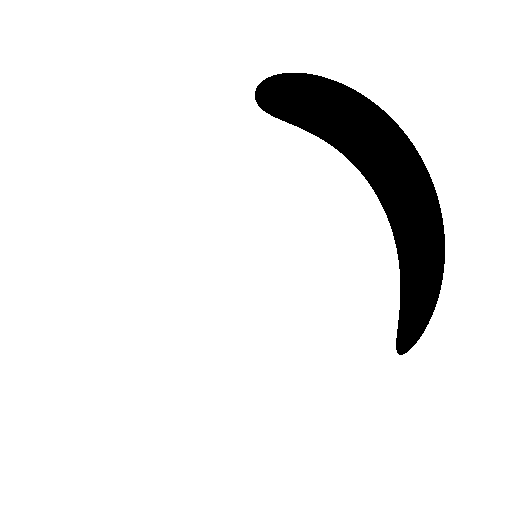
\includegraphics[height=2cm]{images/Z=48.jpg}
  \end{varwidth}
    \quad
  \begin{varwidth}[t]{\textwidth}
    \vspace{0pt}
    
\includegraphics[height=2cm]{images/Z=98.jpg}
  \end{varwidth}
    \quad
  \begin{varwidth}[t]{\textwidth}
    \vspace{0pt}
    
\includegraphics[height=2cm]{images/Z=99.jpg}
  \end{varwidth}
  \caption{6张切片示意图}
  \label{6张切片示意图}
\end{figure}

\section{血管重建}
    \subsection{模型假设}
        \begin{enumerate}
        \item 假设血管无严重扭曲;
        \item 假设管道中轴线与每张切片有且只有一个交点;
        \item 假设球半径固定;
        \item 假设切片间距以及图像象素的尺寸均为1;
        \item 假设切片拍摄不存在误差,数据误差仅与切片数字图像的分辨率有关。
        \end{enumerate}
    \subsection{符号说明}
    \subsection{问题的分析}
        \par
        计算管道的中轴线与半径,给出具体的算法,并绘制中轴线在$XY$、$YZ$、$ZX$平面的投影图。
    \subsection{模型的建立与求解}
        \par
        取坐标系的$z$轴垂直于切片,第1张切片为平面$z=0$,第100张切片为平面$z=99$,并以切片左顶点为坐标原点$o$,$z=0$切片面为$xoy$面建立坐标系$oxyz$,如图(\ref{血管重建坐标系示意图})所示
            \begin{figure}[H]
            \centering
            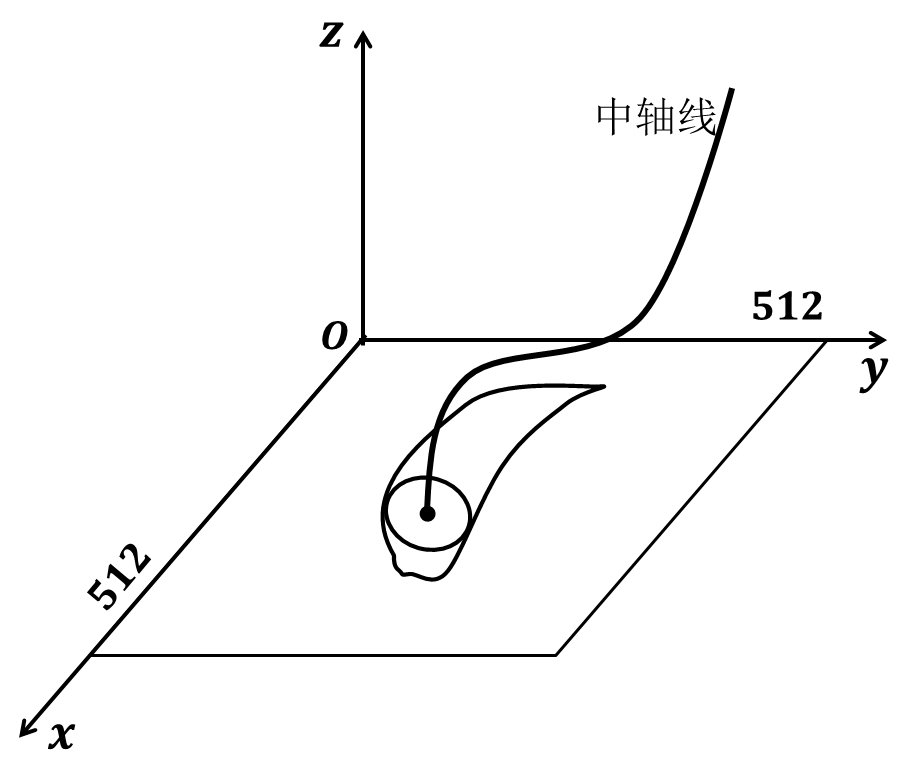
\includegraphics[height=4cm]{images/Reconstruction_of_blood.jpg}
            \caption{血管重建坐标系示意图}
            \label{血管重建坐标系示意图}
            \end{figure}
        \par
        如果我们想重构三维空间中的血管,我们就必须要知道滚动球的大小以及中轴线。就单一切面而言,我们需要求解球心坐标以及球半径,我们对单一切面进行分析,如图(\ref{单一切面坐标系})所示
            \begin{figure}[H]
            \centering
            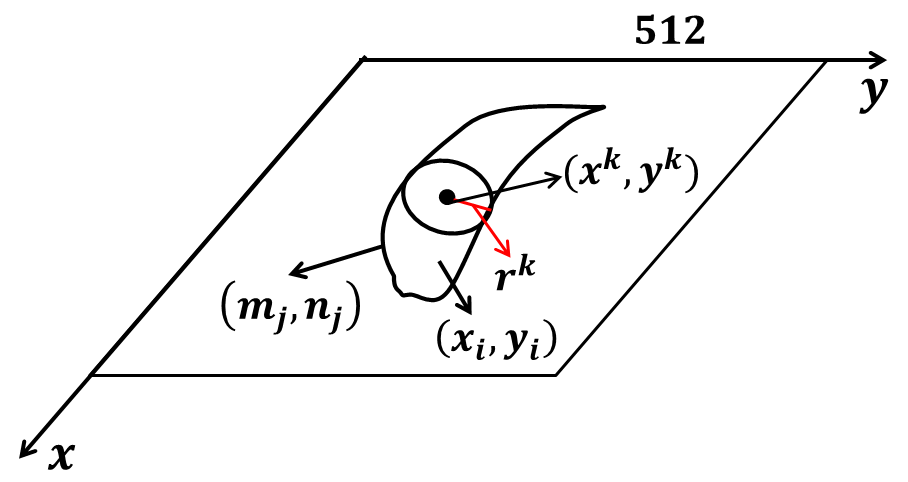
\includegraphics[height=4cm]{images/single_facet_coordination_system.jpg}
            \caption{单一切面坐标系}
            \label{单一切面坐标系}
            \end{figure}
        \par
        我们共有100张切片,第$k$个切片的球中心为$(x^k,y^k)$,球半径为$r^k$。下面,我们的主要工作就是求解$x^k,y^k,r^k$,即切片的最大内切圆。对切片内部任意一个点$(x_i,y_i)$,求出它到轮廓线上所有点$(m_j,n_j)$的距离,并取其最小值,由于所有内点都对应一个最小值,在这些最小值中取最大值,即为:最大内切圆的半径。假设切片内部有$p$个点,第$i$个点的坐标为 $(x_i,y_i)$,切片轮廓线上有$q$个点,第$j$个点的坐标为$(m_j,n_j)$,则切片内部第$i$点到轮廓线上第$j$点的距离为
        \begin{align*}
        d_{i,j} = \sqrt{(x_i-m_j)^2+(y_i-n_j)^2}
        \end{align*}
        第$i$个点对应的最小距离$r_i$ 为
        \begin{align*}
        r_i = \min_j\ d_{ij}
        \end{align*}
        其中:$j = 1,2,\dots,q$。最大内切圆半径为
        \begin{align*}
        r^k = \max_{i}\ r_i
        \end{align*}
        其中:$k = 1,2,\dots,100$为切片序号。将100个切片所对应的最大内切圆半径求取平均值,即为:血管的半径
        \begin{align*}
        r = \frac{1}{100}\sum_{k=1}^{100} r^k
        \end{align*}
        \par
        在求解出中轴线及球的大小之后,我们就可以重建血管了。我们用函数拟合的方法来求解中轴线函数,并拟合中轴线在3个平面上的投影。这里我们不介绍函数拟合的方法。

    \subsection{程序}
        \par
        \begin{lstlisting}[language = Matlab]
        %%%%%%%%%%%%%%%%%%%%%血管重建主程序%%%%%%%%%%%%%%%%%%%%%%
        %% %%%%%%%%%%%%%%%%%%求解最大内切圆%%%%%%%%%%%%%%%%%%
        %[m, medg] = read_qiepian; %读取切片数据
        clc, clear
        load('100pic.mat')
        %计算100张切片的圆心坐标,将其记录在jieguo中的前两列,半径记录在jieguo中的第三列
        jieguo = zeros(100, 3);
        for k = 1:100
            section = m(:,:,k);
            [x, y, r] = MaxInCircle(section);% 求解每个切片的内切圆半径坐标x^k,y^k,及半径r^k
            jieguo(k, 1) = x;
            jieguo(k, 2) = y;
            jieguo(k, 3) = r;
        end
        save('jieguo.mat', 'jieguo')
        %% %%%%%%%%%%%%%%%%%%求中轴线的拟合曲线及其在三个坐标平面的投影%%%%%%%%%%%%%%%%%%
        % 1.绘制中轴线
        figure
        z = (1:100);
        plot3(jieguo(:, 1)', jieguo(:, 2)',z, 'ro');
        hold on
        % 拟合中轴线
        p1 = polyfit((1: 100)', jieguo(:, 2), 6);
        p2 = polyfit((1: 100)', jieguo(:, 1), 8);
        x = p1(1)*z.^6+p1(2)*z.^5+p1(3)*z.^4+p1(4)*z.^3+p1(5)*z.^2+p1(6)*z+p1(7);
        y = p2(1)*z.^8+p2(2)*z.^7+p2(3)*z.^6+p2(4)*z.^5+p2(5)*z.^4+p2(6)*z.^3+p2(7)*z.^2+p2(8)*z+p2(9);
        plot3(y, x, z, 'b')
        grid on
        xlabel x, ylabel y, zlabel z
        legend('中轴线', '拟合中轴线')
        title('拟合中轴线')
        hold off

        % 2.中轴线在xoz面上的投影
        figure
        plot(jieguo(:, 2)', z, 'ro');
        hold on
        % 拟合中轴线在xoz面上的投影
        p = polyfit((1:100)', jieguo(:, 2), 6);  %以6次多项式拟合,横坐标是1到100
        x = p(1)*z.^6+p(2)*z.^5+p(3)*z.^4+p(4)*z.^3+p(5)*z.^2+p(6)*z+p(7);
        plot(x, z, 'b')
        grid on
        xlabel x, ylabel z
        legend('xoz上的投影','拟合xoz上投影')
        title('拟合中轴线在xoz上投影')
        hold off

        % 3.中轴线在yoz面上的投影
        figure
        plot(jieguo(:, 1)', z, 'ro');
        hold on
        % 拟合中轴线在yoz面上的投影
        p = polyfit((1:100)', jieguo(:, 1), 8); % 以8次多项式拟合,横坐标是1到100
        y = p(1)*z.^8+p(2)*z.^7+p(3)*z.^6+p(4)*z.^5+p(5)*z.^4+p(6)*z.^3+p(7)*z.^2+p(8)*z+p(9);
        plot(y, z, 'b')
        xlabel y, ylabel z
        legend('yoz面上的投影', '拟合yoz面上的投影')
        grid on
        title('拟合中轴线在yoz上投影')
        hold off

        % 4.中轴线在xoy面上的投影
        figure
        plot(jieguo(:, 1)',jieguo(:, 2)','ro');
        hold on
        % 拟合中轴线在xoy面上的投影
        p1 = polyfit((1:100)',jieguo(:,2),6);
        p2 = polyfit((1:100)',jieguo(:,1),8);
        x = p1(1)*z.^6+p1(2)*z.^5+p1(3)*z.^4+p1(4)*z.^3+p1(5)*z.^2+p1(6)*z+p1(7);
        y = p2(1)*z.^8+p2(2)*z.^7+p2(3)*z.^6+p2(4)*z.^5+p2(5)*z.^4+p2(6)*z.^3+p2(7)*z.^2+p2(8)*z+p2(9);
        plot(y, x, 'b')
        grid on
        xlabel x, ylabel y
        legend('xoy面上的投影', '拟合xoy面上的投影')
        title('拟合中轴线在xoy上投影')
        %%%%%%%%%%%%%%%%%%带有拟合中轴线的轮廓切面图空间效果图%%%%%%%%%%%%%%%%%%
        clc;clear;close all;
        load('100pic.mat');load('jieguo.mat');
        n=100;m1=size(m,1);m2=size(m,2);
        n=zeros(m1,m2,n);
        for k=0:99
            n(:,:,k+1)=edge(m(:,:,k+1));
        end
        for k=0:5:99
            for i=1:2:512
                for j=1:2:512
                    if (n(i,j,k+1)==1)
                        plot3(i-257,j-257,k+1,'b.');hold on
        end,end,end,end
        hold on

        p1=polyfit((1:100)',jieguo(:,2),6);
        p2=polyfit((1:100)',jieguo(:,1),8);
        z=(1:100);
        x=p1(1)*z.^6+p1(2)*z.^5+p1(3)*z.^4+p1(4)*z.^3+p1(5)*z.^2+p1(6)*z+p1(7);
        y=p2(1)*z.^8+p2(2)*z.^7+p2(3)*z.^6+p2(4)*z.^5+p2(5)*z.^4+p2(6)*z.^3+p2(7)*z.^2+p2(8)*z+p2(9);
        plot3(y,x,z,'r')
        grid on
        title('拟合中轴线的轮廓切面图')
        hold off
        %%%%%%%%%%%%%%%%%%%计算平均半径%%%%%%%%%%%%%%%%%%
        load('jieguo.mat');
        r = mean(jieguo(:,3));
        %%%%%%%%%%%%%%%%%%函数对管道表面进行三维重建(透明化处理)%%%%%%%%%%%%%%%%%%
        clc;clear;close all;
        load('100pic.mat');load('jieguo.mat');
        n=100;m1=size(m,1);m2=size(m,2);
        p1=polyfit((1:100)',jieguo(:,2),6);
        p2=polyfit((1:100)',jieguo(:,1),8);
        z=(1:100);
        x=p1(1)*z.^6+p1(2)*z.^5+p1(3)*z.^4+p1(4)*z.^3+p1(5)*z.^2+p1(6)*z+p1(7);
        y=p2(1)*z.^8+p2(2)*z.^7+p2(3)*z.^6+p2(4)*z.^5+p2(5)*z.^4+p2(6)*z.^3+p2(7)*z.^2+p2(8)*z+p2(9);
        r=mean(jieguo(:,3));
        X=[];Y=[];Z=[];
        for t=0:0.5:4*pi;
            xx=cos(t);
            yy=sin(t);
            x1=r*xx+x;
            y1=r*yy+y;
            z1=z;
            X=[X;x1];
            Y=[Y;y1];
            Z=[Z;z1];
        end
        figure
        surf(X,Y,Z)
        shading flat
        aa=0.5;
        alpha(aa);
        hold on
        plot3(x,y,z,'r')
        hold off
        grid on
        title('使用surf曲面函数按照拟合中轴线和半径模拟血管')
        \end{lstlisting}
        \par
        求解切片圆心坐标及圆半径的程序MaxInCircle如下
        \begin{lstlisting}[language = Matlab]
        function [x, y, r] = MaxInCircle(section)
        % 此函数用与求解单一切片的最大内切圆圆心坐标x^k,y^k及半径r^k
        %%%%%%输入%%%%%
        % section:单一切片;
        %%%%%%输出%%%%%
        % x:圆心横坐标;
        % y:圆心纵坐标;
        % r:圆半径;
        section = 1 - section;
        BW = edge(section, 'sobel');
        BW2 = bwmorph(section, 'skel', inf);
        [x, y, ~] = find(BW2);  %轮廓内点
        [m, n, ~] = find(BW);  %轮廓边界点
        d = zeros(length(x), length(m));
        r = zeros(length(m), 1);
        for i = 1:length(x)
            for j = 1:length(m)
                d(i, j)=sqrt((x(i)-m(j))^2+(y(i)-n(j))^2);
            end
           r(i) = min(d(i, :)); % 最小半径
        end
        [r, ind] = max(r); % 内切圆半径
        x = x(ind) - 256; % 内切圆横坐标
        y = y(ind) - 256; % 内切圆纵坐标
        \end{lstlisting}
    \subsection{结果}
        \par
        中轴线及其在$xoy,yoz,zox$面上的投影结果如图(\ref{中轴线及其二维投影})所示
           \begin{figure}[H]
                \centering
                \begin{subfigure}[b]{0.4\textwidth}
                    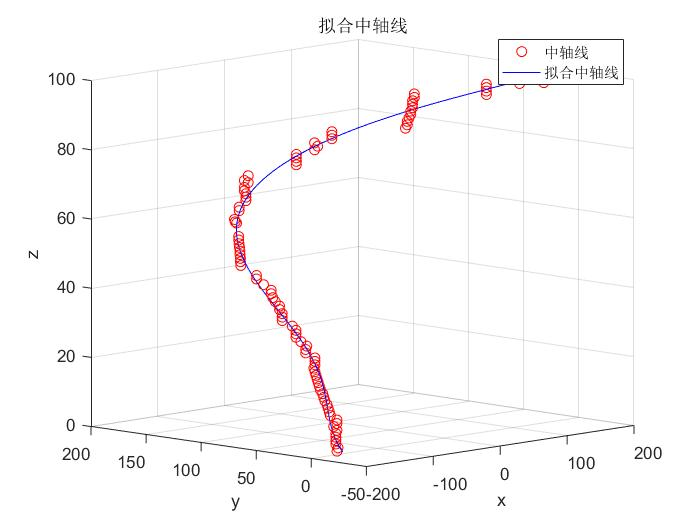
\includegraphics[width=\textwidth]{images/zhongzhouxian.jpg}
                    % \caption{}
                \end{subfigure}
                \begin{subfigure}[b]{0.4\textwidth}
                    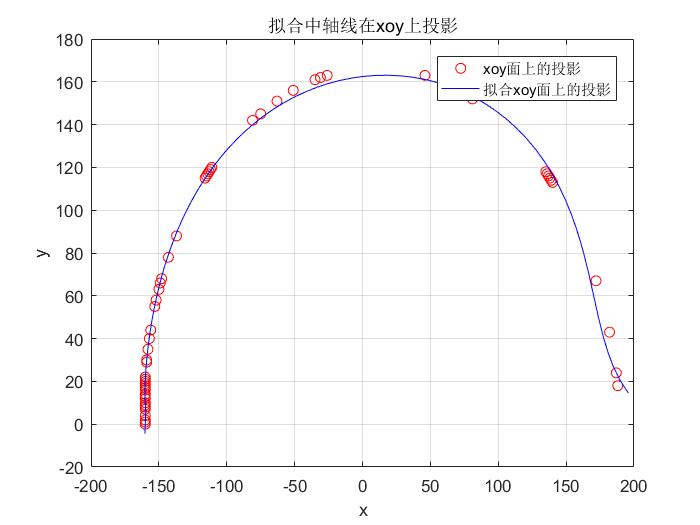
\includegraphics[width=\textwidth]{images/zhongzhouxian_xoy.jpg}
                    % \caption{}
                \end{subfigure}
                \begin{subfigure}[b]{0.4\textwidth}
                    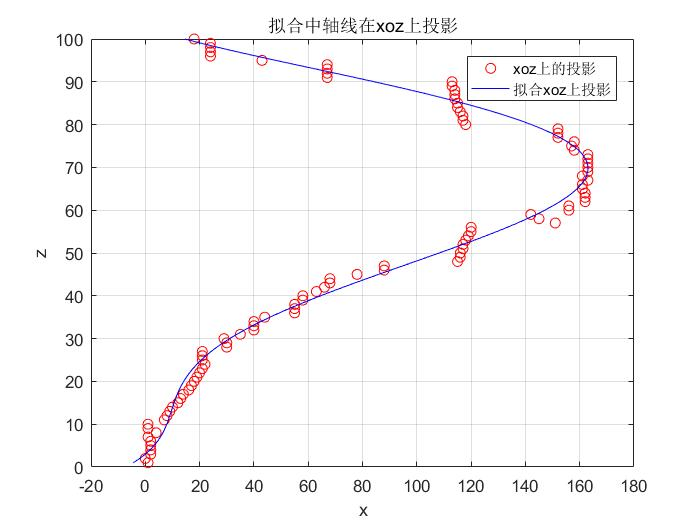
\includegraphics[width=\textwidth]{images/zhongzhouxian_xoz.jpg}
                    % \caption{}
                \end{subfigure}
                \begin{subfigure}[b]{0.4\textwidth}
                    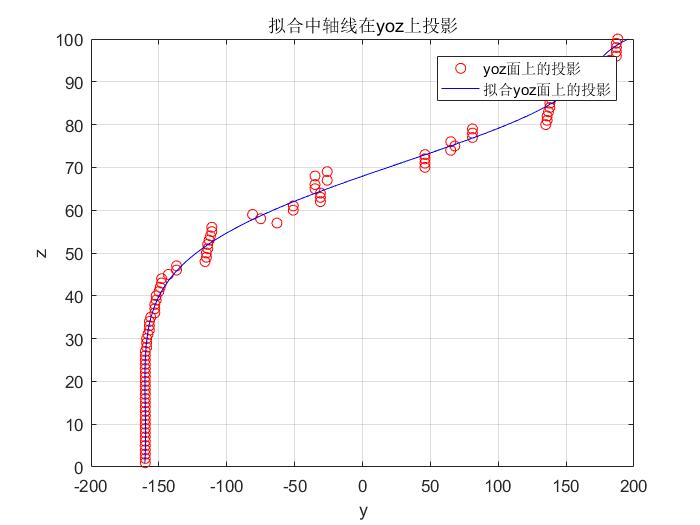
\includegraphics[width=\textwidth]{images/zhongzhouxian_yoz.jpg}
                    % \caption{}
                \end{subfigure}
                \caption{中轴线及其二维投影}
                \label{中轴线及其二维投影}
            \end{figure}
            拟合中轴线的轮廓切面及最终重建的血管如图(\ref{重建血管})所示
           \begin{figure}[H]
                \centering
                \begin{subfigure}[b]{0.4\textwidth}
                    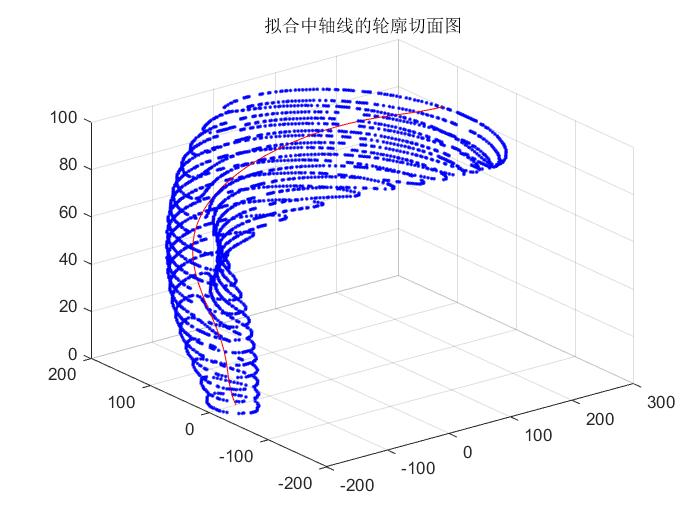
\includegraphics[width=\textwidth]{images/lunkuoqiemian.jpg}
                    % \caption{}
                \end{subfigure}
                \begin{subfigure}[b]{0.4\textwidth}
                    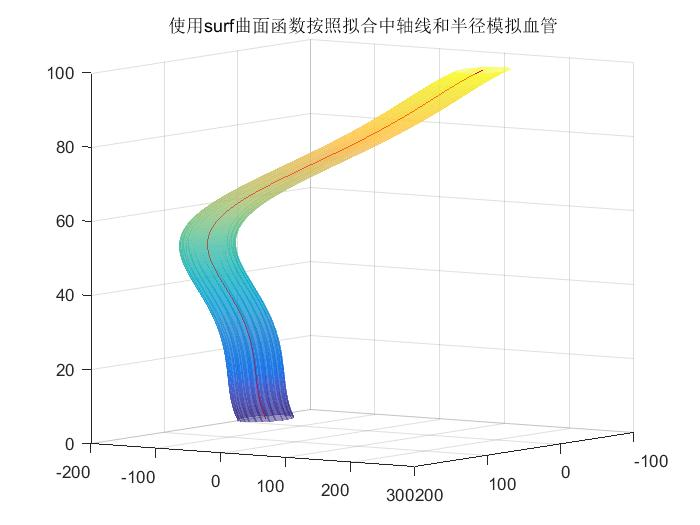
\includegraphics[width=\textwidth]{images/xueguanchongjian.jpg}
                    % \caption{}
                \end{subfigure}
                \caption{重建血管}
                \label{重建血管}
            \end{figure}
% \end{document}
